\def\duedate{\today}
\def\HWnum{1}
\documentclass[10pt,a4paper]{book}

% custom section formatting
\usepackage{titlesec}
\titleformat{\chapter}[display]
{\normalfont\Large\filcenter\sffamily}
{\titlerule[1pt]%
\vspace{1pt}%
\titlerule
\vspace{1pc}%
\LARGE\MakeUppercase{\chaptertitlename} \thechapter}
{1pc}
{\titlerule
\vspace{1pc}%
\Huge}

% appendix handling
\usepackage[toc,page]{appendix}
    
% encoding for file and font
\usepackage[utf8]{inputenc}
\usepackage[T1]{fontenc}

% math formatting/tools
\usepackage{amsmath}
\usepackage{amssymb}
\usepackage{mathtools}
\usepackage[arrowdel]{physics}

% unit formatting
\usepackage{siunitx}
\AtBeginDocument{\RenewCommandCopy\qty\SI}

% figure formatting/tools
\usepackage{graphicx}
\usepackage{float}
\usepackage{subcaption}
\usepackage{multirow}
\usepackage{import}
\usepackage{pdfpages}
\usepackage{transparent}
\usepackage{currfile}

\NewDocumentCommand\incfig{O{1} m}{
    \def\svgwidth{#1\textwidth}
    \import{./Figures/\currfiledir}{#2.pdf_tex}
}

\newcommand{\bef}{\begin{figure}[h!tb]\centering}
\newcommand{\eef}{\end{figure}}

\newcommand{\bet}{\begin{table}[h!tb]\centering}
\newcommand{\eet}{\end{table}}

% hyperlink references 
\usepackage{hyperref}
\hypersetup{
    colorlinks=true,
    linkcolor=blue,
    filecolor=magenta,
    urlcolor=cyan,
    pdftitle={Physics 1 Notes},
    pdfauthor={Richard Whitehill},
    pdfpagemode=FullScreen
}
\urlstyle{same}

\newcommand{\eref}[1]{Eq.~(\ref{eq:#1})}
\newcommand{\erefs}[2]{Eqs.~(\ref{eq:#1})--(\ref{eq:#2})}

\newcommand{\fref}[1]{Fig.~(\ref{fig:#1})}
\newcommand{\frefs}[2]{Fig.~(\ref{fig:#1})--(\ref{fig:#2})}

\newcommand{\aref}[1]{Appendix~(\ref{app:#1})}
\newcommand{\sref}[1]{Section~(\ref{sec:#1})}
\newcommand{\srefs}[2]{Sections~(\ref{sec:#1})-(\ref{sec:#2})}

\newcommand{\tref}[1]{Table~(\ref{tab:#1})}
\newcommand{\trefs}[2]{Table~(\ref{tab:#1})--(\ref{tab:#2})}

% tcolorbox formatting/definitions
\usepackage[most]{tcolorbox}
\usepackage{xcolor}
\usepackage{xifthen}
\usepackage{parskip}

\definecolor{peach}{rgb}{1.0,0.8,0.64}

\DeclareTColorBox[auto counter, number within=chapter]{defbox}{O{}}{
    enhanced,
    boxrule=0pt,
    frame hidden,
    borderline west={4pt}{0pt}{green!50!black},
    colback=green!5,
    before upper=\textbf{Definition \thetcbcounter \ifthenelse{\isempty{#1}}{}{: #1} \\ },
    sharp corners
}

\newcommand*{\eqbox}{\tcboxmath[
    enhanced,
    colback=black!10!white,
    colframe=black,
    sharp corners,
    size=fbox,
    boxsep=8pt,
    boxrule=1pt
]}

\newtcolorbox[auto counter, number within=chapter]{exbox}{
    parbox=false,
    breakable,
    enhanced,
    sharp corners,
    boxrule=1pt,
    colback=white,
    colframe=black,
    before upper= \textbf{Example \thetcbcounter:}\,,
    before lower= \textbf{Solution:}\,,
    segmentation hidden
}

\newtcolorbox{resbox}{
    enhanced,
    colback=black!10!white,
    colframe=black,
    boxrule=1pt,
    boxsep=0pt,
    top=2pt,
    ams nodisplayskip,
    sharp corners
}


\begin{document}

\prob{1}{
    Consider the scattering of monochromatic photons by free electrons (Compton scattering). \\[3 pt]
    
(a) Assuming that the electron is initially at rest and using energy and momentum conservation, show that the shift in the photon wavelength $\Delta \lambda = \lambda_{f}^{\gamma} - \lambda_{i}^{\gamma}$ is given by
\begin{eqnarray}
    \Delta \lambda = 2 \lambda_{e} \sin^2{\theta_{0}/2}~{\rm with}~\lambda_{e} = \frac{h}{mc}
,\end{eqnarray}
where $m$ is the electron mass, $c$ is the speed of light, and $\theta_0$ is the angle that the momentum of the scattered photon makes with the momentum of the incident photon.
Determine (under the same assumption) the magnitude and direction of the recoil momentum of the electron as a function of the incident-photon energy $E_{i}^{\gamma}$ and scattering angle $\theta_0$.

(b) Assume that the electron has an initial momentum $\va*{p}_{i}$ parallel to the incident-photon momentum $\va*{p}_{i}^{\gamma}$.
Using energy and momentum conservation, show that the wavelength shift is given in this case by
\begin{eqnarray}
    \Delta \lambda = 2 \lambda_{i}^{\gamma} \frac{p_{i}^{\gamma} + p_{i}}{E_{i}/c - p_{i}} \sin^2{\theta/2} 
,\end{eqnarray}
where $\lambda_{i}^{\gamma}$ is the wavelength of the incident photon, $\theta$ is the angle of the scattered photon, and $E_{i} = c^2 \sqrt{p_{i}^2 + (mc)^2}$ is the initial energy of the electron. \\[3 pt]

(c) Show that the result in part (b) above can be derived from the expressions in \\ part (a), where the electron is initially at rest, by a suitable Lorentz transformation.
}

\sol{ 

(a) Consider the reaction $\gamma e \rightarrow \gamma e$ in Fig. \ref{fig:prob1a}.

\begin{figure}[h!tb]
    \centering
    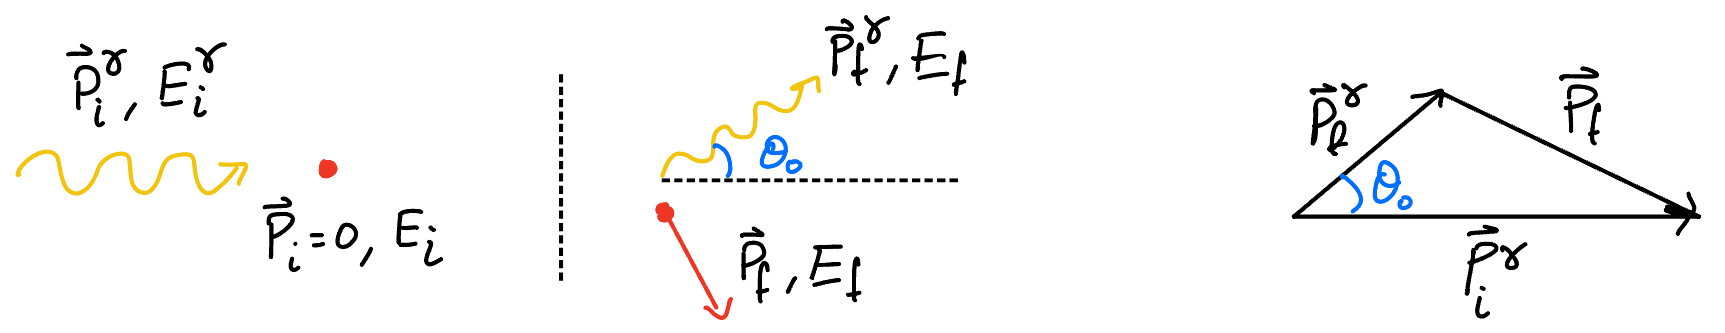
\includegraphics[width=0.7\textwidth]{prob1a.jpeg}
    \label{fig:prob1a}
    \caption{Sketch of the compton scattering process and momentum conservation with electron at rest in the initial state and photon deflecting at angle $\theta_0$ relative to the beam axis.}
\end{figure}

Energy conservation gives that 
\begin{eqnarray}
\label{eq:E-conservation}
    E_{i}^{\gamma} + E_{i} = E_{f}^{\gamma} + E_{f}
.\end{eqnarray}
Note that the energy of the incoming/outgoing photon and electron are given as $E_{i,f}^{\gamma} = p_{i,f}^{\gamma} c$ and $E_{i,f} = c \sqrt{(mc)^2 + p_{i,f}^2}$, respectively.
Using these, Eq. (\ref{eq:E-conservation}) becomes
\begin{eqnarray}
    p_{i}^{\gamma}c + mc^2 = p_{f}^{\gamma}c + c\sqrt{(mc)^2 + p_{f}^2}
.\end{eqnarray}
Dividing through by $c$, subtracting $p_{f}^{\gamma}$ on both sides, and squaring, we obtain
\begin{eqnarray}
    \label{eq:E-conservation-intermediate}
    (m c)^2 + p_{f}^2 = [(p_{i}^{\gamma} - p_{f}^{\gamma}) + mc]^2 = (p_{i}^{\gamma} - p_{f}^{\gamma})^2 + (mc)^2 - 2(p_{i}^{\gamma} - p_{f}^{\gamma}) mc
.\end{eqnarray}

Now, note that momentum conservation tells us that $\va*{p}_{i}^{\gamma} = \va*{p}_{f}^{\gamma} + \va*{p}_{e}'$, and thus,
\begin{eqnarray}
    p_{f}^2 = (\va*{p}_{i}^{\gamma} - \va*{p}_{f}^{\gamma})^2 = (p_{i}^{\gamma})^2 + (p_{f}^{\gamma})^2 - 2 \va*{p}_{i}^{\gamma} \cdot \va*{p}_{f}^{\gamma}
.\end{eqnarray}
Using this, Eq. \ref{eq:E-conservation-intermediate} becomes
\begin{eqnarray}
    - 2 p_{i}^{\gamma} p_{f}^{\gamma} \cos{\theta_0} = -2 p_{i}^{\gamma} p_{f}^{\gamma} - 2 (p_{i}^{\gamma} - p_{f}^{\gamma}) mc
,\end{eqnarray}
and dividing through by $p_{i}^{\gamma} p_{f}^{\gamma}$ after substituting $p_{i,f}^{\gamma} = h/\lambda_{i,f}$ and rearranging we arrive at the desired solution:
\begin{eqnarray}
    \label{eq:1a-result}
    \begin{aligned}
        &\frac{1}{p_{f}^{\gamma}} - \frac{1}{p_{i}^{\gamma}} = \frac{1}{mc}(1 - \cos{\theta_0}) \\
        &\eqbox{ \Delta \lambda = \lambda_{f} - \lambda_{i} = \frac{h}{mc} (1 - \cos{\theta_0}) }
    .\end{aligned}
\end{eqnarray}
Note that $1 - \cos{\theta_0} = 1 - (\cos^2{\theta_0/2} - \sin^2{\theta_0/2}) = 2 \sin^2{\theta_0/2}$.



(b) If the electron is moving collinearly and in the same direction as $\gamma$ before the interaction, energy conservation reads
\begin{eqnarray}
    p_{i}^{\gamma} + \frac{E_{i}}{c} = p_{f}^{\gamma} + \sqrt{(mc)^2 + p_{f}^2}
.\end{eqnarray}

\begin{figure}[h!tb]
    \centering
    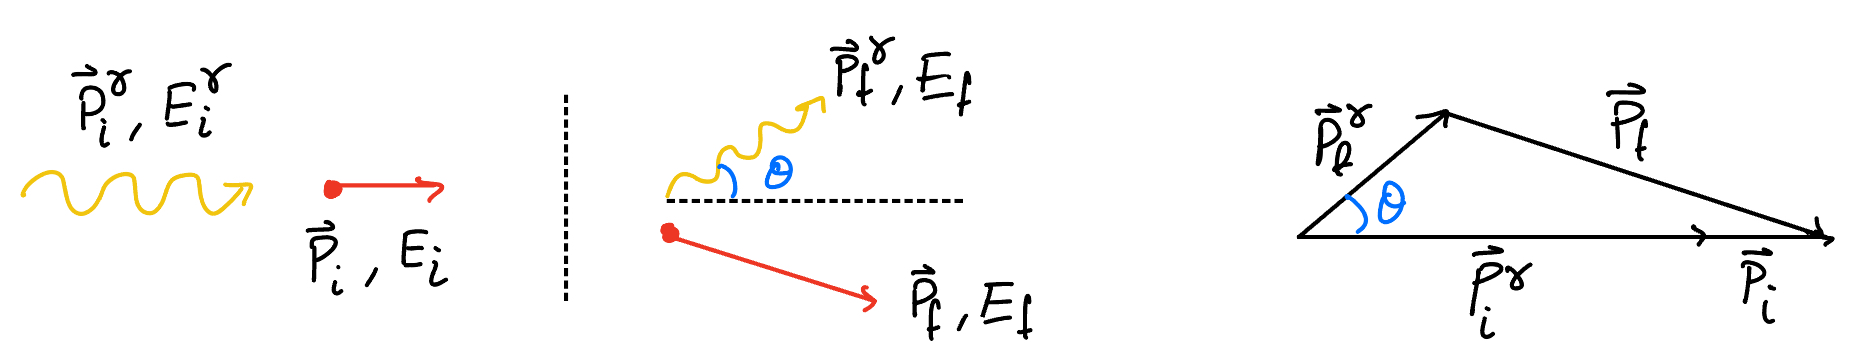
\includegraphics[width=0.7\textwidth]{prob1b.jpeg}
    \label{fig:prob1b}
    \caption{Sketch of compton scattering process with electron with momentum $p_{i}$ in the initial state and photon deflecting at angle $\theta_0$ relative to the beam axis.}
\end{figure}


The manipulations are much the same since $p_{i}$ is a known parameter (and also therefore $E_{i}$).
\begin{eqnarray}
    \label{eq:1b-result}
    \begin{aligned}
        (mc)^2 + p_{f}^2 &= (p_{i}^{\gamma} - p_{f}^{\gamma})^2 + (mc)^2 + p_{i}^2 + 2 \Big( \frac{E_{i}}{c} \Big) (p_{i}^{\gamma} - p_{f}^{\gamma}) \\
        [\va*{p}_{i} + \va*{p}_{i}^{\gamma} - \va*{p}_{f}^{\gamma}]^2 &= (p_{i}^{\gamma} - p_{f}^{\gamma})^2 + p_{i}^2 - 2 \Big( \frac{E_{i}}{c} \Big) (p_{f}^{\gamma} - p_{i}^{\gamma}) \\
        \va*{p}_{i} \cdot \va*{p}_{i}^{\gamma} - \va*{p}_{i} \cdot \va*{p}_{f}^{\gamma} - \va*{p}_{i}^{\gamma} \cdot \va*{p}_{f}^{\gamma} &= - p_{i}^{\gamma} p_{f}^{\gamma} - \frac{E_{i}}{c} (p_{f}^{\gamma} - p_{i}^{\gamma}) \\
        p_{i} p_{i}^{\gamma} - p_{i} p_{f}^{\gamma} \cos{\theta} - p_{i}^{\gamma} p_{f}^{\gamma} \cos{\theta} &= -p_{i} p_{f}^{\gamma} - \frac{E_{i}}{c} (p_{f}^{\gamma} - p_{i}^{\gamma}) \\
        \frac{E_{i}}{c} \Big( \frac{1}{p_{f}^{\gamma}} - \frac{1}{p_{i}^{\gamma}} \Big) &= \frac{p_{i}}{p_{f}^{\gamma}} - \frac{p_{i}}{p_{i}^{\gamma}} + (1 - \cos{\theta}) \\
        \Big( \frac{E_{i}}{c} - p_{i} \Big) \Big( \frac{1}{p_{f}^{\gamma}} - \frac{1}{p_{i}^{\gamma}} \Big) &= 2 \Big( \frac{p_{i}}{p_{i}^{\gamma}} + 1 \Big) \sin^2{\theta/2} \\
        \frac{1}{p_{f}^{\gamma}} - \frac{1}{p_{i}^{\gamma}} &= 2 \Big( \frac{1}{p_{i}^{\gamma}} \Big) \frac{p_{i} + p_{i}^{\gamma}}{E_{i}/c - p_{i}} \sin^2{\theta/2} \\
                                                            &\eqbox{ \Delta \lambda = 2 \lambda_{i}^{\gamma} \frac{p_{i} + p_{i}^{\gamma}}{E_{i}/c - p_{i}} \sin^2{\theta/2} }
    .\end{aligned}
\end{eqnarray}

(c) We can transform from the result Eq. (\ref{eq:1a-result}) in part (a), where the electron is initially at rest, to the result of part (b), given by Eq. (\ref{eq:1b-result}), via a suitable Lorentz transformation.

\begin{figure}[h!tb]
    \centering
    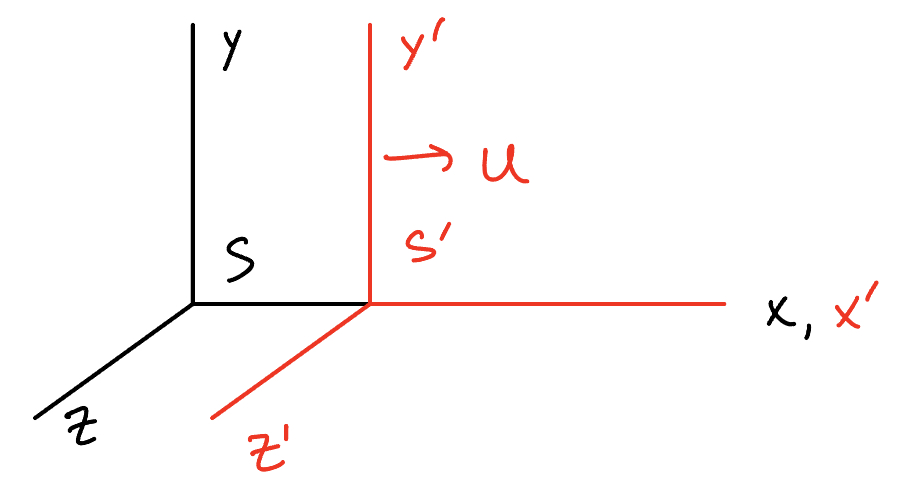
\includegraphics[width=0.5\textwidth]{prob1c.jpeg}
    \label{fig:prob1c}
    \caption{Skeach of Lorentz transformation between frames $S$ and $S'$ moving with relative velocity $u$.}
\end{figure}

Let $S$ be the frame for part (b), where the electron has momentum $p_{i}$ in the initial state, and $S'$ be the frame for part (a), where the electron is at rest in the initial state.
The Lorentz transformation of any 4-vector $a$ from $S'$ to $S$ is given as
\begin{eqnarray}
\label{eq:lorentz-transform}
   \begin{cases}
   c a^{0} = \gamma (c a'^{0} + \beta a'^{x}) \\
   a^{x}  = \gamma (a'^{x} + \beta a'^{0}) \\
   a^{y,z} = a'^{y,z}
   \end{cases} 
.\end{eqnarray}
where the Lorentz factor $\gamma = [1 - \beta^2]^{-1/2}$, where $\beta$ is the velocity of the electron in $S$ (normalized to $c$).
Note that $\gamma^2 = 1 + [p_{i}/(mc)]^2$

Using \eref{lorentz-transform} for the energy of the photon we find
\begin{align}
    \label{eq:initial-transform}
    E_{i}^{\gamma} &= \gamma ( E_{i}'^{\gamma} + \beta p_{i,x}'^{\gamma} ) = \gamma E_{i}'^{\gamma} (1 + \beta) \\
    \label{eq:final-transform}
    E_{f}^{\gamma} &= \gamma E_{f}'^{\gamma} (1 + \beta \cos{\theta_0})
.\end{align}

Now, we can write $E_{i,f}^{\gamma} = c p_{i,f}^{\gamma} = hc/\lambda_{i,f}^{\gamma}$.
Hence, \erefs{initial-transform}{final-transform} tell us how the wavelengths of the initial and final state photon transform between the $S$ and $S'$\footnote{As a sanity check these should reduce to the doppler shift.}:
\begin{align}
    \frac{1}{\lambda_{i}^{\gamma}} &= \frac{\gamma}{\lambda_{i}'^{\gamma}} (1+\beta) \\
    \frac{1}{\lambda_{f}^{\gamma}} &= \frac{\gamma}{\lambda_{f}'^{\gamma}} (1+\beta \cos{\theta_0})
.\end{align}

All that remains is to transform the factor $\cos{\theta_0}$ from $S$ to $S'$.
By definition,
\begin{eqnarray}
    p_{f,x}'^{\gamma} = p_{f}'^{\gamma} \cos{\theta_0} = \frac{E_{f}'^{\gamma}}{c} \cos{\theta_0}
.\end{eqnarray}
Using this equation, we can use the Lorentz transformation to find
\begin{eqnarray}
    \begin{aligned}
        \gamma ( p_{f,x}^{\gamma} - \frac{\beta}{c} E_{f}^{\gamma} ) &= \frac{\gamma E_{f}^{\gamma} ( 1 - \beta \cos{\theta} )}{c} \cos{\theta_0} \\
    \cos{\theta_0} &= \frac{\cos{\theta} - \beta}{1 - \beta \cos{\theta}}
    .\end{aligned}
\end{eqnarray}

Plugging the expressions for $\lambda_{i,f}^{\gamma}$ and $\cos{\theta_0}$

}






\prob{2}{
After the discovery of the electron by Thomson in 1897, it was believed that ``atoms were like puddings, with negatively charged electrons stuck in like raisins in a smooth background of positive charge'' (S. Weinberg).
This picture was drastically changed by experiments performed by Rutherford and collaborators, who scattered $\alpha$ particles ($^{4}{\rm He}$ nuclei, which we now know consist of two protons and two neutrons bound together by the nuclear force, having electric charge $2e$) off a thin foil of gold. They observed $\alpha$ particles scattered at large backward angles.
This was totally unexpected, since electrons are much lighter than $\alpha$ particles. \\[3pt]

(a) Consider a particle of mass $M$ and velocity $v$ hitting a particle of mass $m$ at rest and continuing along the same line with velocity $v'$.
Show that, for a given $v$, energy and momentum conservation lead to two possible solutions for $v'$.
If a certain condition is satisfied, one of these solutions corresponds to the case in which particle $M$ inverts its direction of motion.
What is this condition? \\[3pt]

(b) Suppose the $\alpha$ particles (which were in fact emitted by a radium source in Rutherford's experiment) have velocity $v \approx \SI{2.1e9}{\centi\metre\per\second}$, and that the target particles (much heavier than the $\alpha$ particles) have each charge $Ze$.
If the $\alpha$'s and target particles interact via the Coulomb repulsion, what is the distance of closest approach?
Show that this distance is of the order $3Z \times 10^{-14}~\SI{}{\centi\metre}$, and therefore (even for $Z \approx 100$) much smaller than atomic radii.

}




\end{document}
